\newthought{Countable sets} and counting schemes for infinite countable sets are the topics of the problem in this note. \index{countable set}

\vspace{10 mm}
\begin{problem}
Let $P = \{ N \subset \mathbb{N}: N \text{  finite}\}$. Prove $P$ is countable.	     
\end{problem}

Let's revisit what it means for an infinite set to be countable: An infinite set $M$ is countable if there is a bijection \footnote{A bijection is a function that is one-to-one and onto.} from $M$ to $\mathbb{N}$. 

Given this definition, the problem statement is quite remarkable: the set of all the finite subsets of $\mathbb{N}$ is not ``bigger'' than $\mathbb{N}$.
\newline

\noindent Our strategy will be to start smaller and prove certain subsets of $P$ are countable. We then expand it to $P$. We start by proving that the set of all subsets of $\mathbb{N}$ of size two is countable. We actually will prove something stronger, namely the set of ordered pairs of natural numbers is countable.

\begin{thm}\label{countingpairs}
The set of ordered pairs $\mathbb{N} \times \mathbb{N}$ is countable.
\end{thm}

\todo{Mention puzzle 136 (Catching a Spy) from Levitin: Algorithmic Puzzles}

\begin{proof}
We need a bijection from $\mathbb{N} \times \mathbb{N} \rightarrow \mathbb{N}$. There are many ways to do this 
\footnote{A very elegant way is described at \url{http://www.math.upenn.edu/~wilf/website/recounting.pdf}}.

\begin{marginfigure}[1.0in]
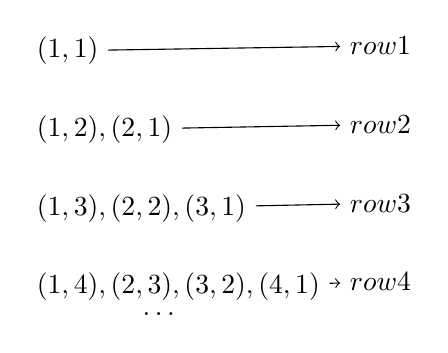
\begin{tikzpicture}
 \node at (-2, 3)  (1l) [anchor=north west] {$(1, 1)$};
 \node at (3, 3)  (1r) [anchor=north east] {$\text{row } 1$};
 \node at (-2, 2)  (2l) [anchor=north west] {$(1, 2), (2, 1)$};
 \node at (3, 2)  (2r) [anchor=north east] {$\text{row } 2$};
 \node at (-2, 1)  (3l) [anchor=north west] {$(1, 3), (2, 2), (3, 1)$};
 \node at (3, 1)  (3r) [anchor=north east] {$\text{row } 3$};
 \node at (-2, 0)  (4l) [anchor=north west] {$(1, 4), (2, 3), (3, 2), (4, 1)$};
 \node at (3, 0)  (4r) [anchor=north east] {$\text{row } 4$};
 \node at (0, -0.5) [anchor=north east] {$\dots$};
 \draw [->] (1l) -- (1r);
 \draw [->] (2l) -- (2r);
 \draw [->] (3l) -- (3r);
 \draw [->] (4l) -- (4r);
\end{tikzpicture}
\caption{Counting all pairs.}
\label{fig:counting}
\end{marginfigure}

The main idea we are going to use for our bijection is to order the pairs $(i, j) \in \mathbb{N} \times \mathbb{N}$ in rows, such that each pair in a row has the same value when summing the components of the pair. Figure \ref{fig:counting} illustrates the idea. Row one has all pairs with components that sum up to two (in this case only one pair). Row two has all pairs with components that sum up to three, row three all pairs which sum to four, $\dots$. Notice also that
in a row the pairs are sorted in increasing order of the first component.

We count the pairs from left to right in each row and go down the rows starting at the first row. For a given pair $(i, j)$, how many pairs come before it in our counting scheme? It is in row $i + j - 1$, so there are $k: 1 \le k < i + j - 1$ rows before it.  Each row $k$ has $k$ pairs in it. This means there are
$$
\sum_{k=1}^{i+j-2} k = \frac{(i+j-2)(i+j-1)}{2}
$$
pairs in rows before our pair $(i, j)$. There are $i - 1$ pairs before $(i, j)$ in the same row. Therefore, our counting function is 
$$
f:\mathbb{N} \times \mathbb{N} \rightarrow \mathbb{N}, ~~f(i, j) = i + \frac{(i+j-2)(i+j-1)}{2}
$$
Suppose we have two pairs $(i_1, j_1) \ne (i_2, j_2)$. We have two cases:

\begin{itemize}
\item $i_1+j_1=i_2+j_2$, same row, then $i_1 \ne i_2$, so $f(i_1, j_1) \ne f(i_2, j_2)$
\item $i_1+j_1 \ne i_2+j_2$, different rows, so $f(i_1, j_1) \ne f(i_2, j_2)$
\end{itemize}

This means, $f$ is one-to-one.

To prove that $f$ is onto, we consider an arbitrary $n \in \mathbb{N}$ and find a pair $(i, j)$ with $f(i, j)=n$. Working backwards and assuming we have a pair $(i, j)$ with $f(i, j)=n$, it would fall on a row $r = i + j - 1$. In each row $k$ there are $k$ pairs, $n$ is on row $r$, so
$$
\sum_{k=1}^{r-1} k = \frac{r(r-1)}{2} < n \leq \sum_{k=1}^{r} k = \frac{r(r+1)}{2}
$$
Solving for $r$ we have:\footnote{Note that $\frac{1 + \sqrt{1 + 8 n}}{2} - \frac{-1 + \sqrt{1 + 8 n}}{2} = 1$}

$$
r^2 - r - 2n < 0, ~~r^2 + r - 2n \geq 0, ~~r = \bigg\lceil \frac{-1 + \sqrt{1 + 8 n}}{2} \bigg\rceil
$$
And then
$$
i = n - \frac{r(r - 1)}{2}, ~~j = r - i + 1
$$
This means that given an arbitrary $n$, there exists a pair $(i, j)$ with $f(i, j)=n$, so $f$ is onto.

It follows that $f$ is a bijection and $\mathbb{N} \times \mathbb{N}$ is countable.
\end{proof}

A corrollary to Theorem~\ref{countingpairs} let's us expand the countable subsets of $P$ even more.

\begin{cor}
Set of all finite sequences of length $k$, $\mathbb{N}^k$ is countable.\footnote{$\mathbb{N}^k$ is the set of sequences of length k, or the cartesian product 
$\mathbb{N} \times \mathbb{N} \times \dots \mathbb{N}$. The set of pairs is $\mathbb{N}^2=\mathbb{N} \times \mathbb{N}$.}
\end{cor}

\begin{proof}
Follows by induction on $k$: Assuming $\mathbb{N}^{k - 1}$ is countable, then
$$
\mathbb{N}^k = \mathbb{N}^{k - 1} \times \mathbb{N}
$$
is also countable according to Theorem~\ref{countingpairs}.
\end{proof}

From the corrollary we now know\footnote{We keep using the fact that the set of all finite subsets of $\mathbb{N}$ of size $k$ is a subset of the set of all sequences of size $k$. To see this impose an order on a set of size $k$ and you get a sequence.} that the set of all subsets of $\mathbb{N}$ of size $k$ is countable (it's a subset of $\mathbb{N}^k$). The problem in this section asks us to prove that $P$ is countable, which means the union of all these countable sets is countable. The next theorem will prove just that.

\begin{thm}
Let $A_n, ~n \in \mathbb{N}$ be countable sets. Then 
$$
\bigcup_{n=1}^\infty A_n
$$ 
is countable\footnote{Exercise 1.5.3 on page 30 from \bibentry{abbott15}.}.
\end{thm}

\begin{proof}
$A_n$ is countable, so there exists a bijection $f_n:\mathbb{N} \rightarrow A_n$. We already know that $\mathbb{N} \times \mathbb{N}$ is countable, so there exists a bijection $g:\mathbb{N} \rightarrow \mathbb{N} \times \mathbb{N}$.

We define $F:\mathbb{N} \rightarrow \bigcup_{n=1}^\infty A_n$
$$
F(n) = f_i(j), ~\text{where}~ (i, j) = g(n)
$$
We claim that $F$ is a bijection.

Take $n_1 \ne n_2$. Then $g(n_1) \ne g(n_2)$ and $(i_1, j_2) \ne (i_2, j_2)$, so 
$$
f_{i_1}(j_1) \ne f_{i_2}(j_2)
$$
It means $F(n_1) \ne F(n_2)$ and $F$ is one-to-one.

Now pick an arbitrary $a \in \bigcup_{n=1}^\infty A_n$. Then there exists $i \in \mathbb{N}$ with $a \in A_i$. \footnote{We assume here the $A_i$ are disjoint, if not we make them disjoint and their union stays the same.} There also exists $j \in \mathbb{N}$ with $f_i(j) = a$. The pair $(i, j)$ is in
$\mathbb{N} \times \mathbb{N}$, so there exists $n \in \mathbb{N}$ with $g(n)=(i, j)$. It follows that $F(n)=a$ and F is onto. 
\end{proof}

Let us use this last theorem to prove the following statement\footnote{Exercise 0.0.1 on page xiii from \bibentry{tao2021introduction}.}:

\begin{thm}
If $(x_\alpha)_{\alpha \in A}$ is a collection of numbers $(x_\alpha) \in [0, +\infty]$ such that $\sum_{\alpha \in A} x_\alpha < \infty$, then $x_\alpha = 0$ for all but at most countably many $\alpha \in A$, even if $A$ itself is uncountable.
\end{thm}

\begin{proof}

We adopt the same definition of sum over the collection of numbers as in Terence Tao's book:

$$
\sum_{\alpha \in A} x_\alpha = \sup\{\sum_{\alpha \in F} x_\alpha: F \subset A, F \text{ finite}\}
$$

We will use the harmonic series $\sum_{n=1}^\infty \frac{1}{n}$ as our yardstick. For each $n \in \mathbb{N}$ we define the subset $A_n \subset A$:

$$
A_n = \{\alpha: \alpha \in A, x_\alpha \geq \frac{1}{n}\}
$$

The sets $A_n$ have to be finite because otherwise the sum $\sum_{\alpha \in A_n} x_\alpha$ would be an infinite sum bigger than the harmonic series, so it would diverge which is a contradiction to $\sum_{\alpha \in A} x_\alpha < \infty$.

We also know that $\bigcup_{n=1}^\infty A_n$ collect all the non-zero elements $x_\alpha$ and according to the previous theorem this union is countable. 
\end{proof}